%!TEX root = ../main.tex
\chapter{Imágenes a Color}
\label{chap:color}
En este capítulo se definen los conceptos básicos de imágenes digitales, así también los espacios de color utilizados en este trabajo. 

\section{Imágenes Digitales}
El píxel es la unidad básica de una imagen digital. Un píxel contiene información sobre el punto de color. Para poder visualizar, almacenar y procesar dicha información, se debe conocer el espacio de color en el cual está representado.

\addsymbol{symbol:F}
\addsymbol{symbol:e}
\addsymbol{symbol:d}
\addsymbol{symbol:n}
Una imagen digital consiste en un conjunto de píxeles. La definición formal esta dada como $F:e\rightarrow d$, donde $e$ es un subconjunto discreto de una grilla rectangular $\mathbb{N}^{2}$ para imágenes en dos dimensiones y $d$ es el rango de valores permitidos para el píxel.
Los píxeles de imágenes binarias se representan con un único valor en un rango de [0, 1]. Las imágenes en escala de grises utilizan un valor en el rango de [0, 255] como un subconjunto de $\mathbb{Z}$. Un píxel tiene asociado un color que se representa con un vector $(V_{1},V_{2},V_{3},...,V_{n})$ donde $n$ es el número de dimensiones del vector. 
\subsection{Espacios de Color}
Muchos espacios de color existen en el estado del arte. En esta sección se explican los espacios de color utilizados en este trabajo.
\subsubsection{RGB}
\addsymbol{symbol:r} \addsymbol{symbol:g} \addsymbol{symbol:b}
El espacio de color \gls{rgb} está especificado mediante cantidades positivas de los colores primarios, rojo ($r$), verde ($g$) y azul($b$), formando un cubo en el espacio 3D como se muestra en la Figura \ref{img:rgb-diagrama}. 
\begin{figure}[h!]
\centering
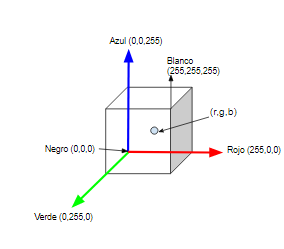
\includegraphics[width=80mm]{./figuras/diagrama-rgb.png}
\caption{Representación espacial del modelo de color RGB}
\label{img:rgb-diagrama}
\end{figure}
El espacio de color RGB es el que se emplea más comúnmente, es dependiente del dispositivo y se basa en la síntesis aditiva, en la cual un color puede ser representado mediante la mezcla por adición de los colores primarios~\cite{OrtizZamora2002}.
\begin{figure}[h!]
\centering
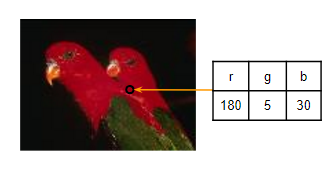
\includegraphics[width=80mm]{./figuras/ejemplo-rgb.png}
\caption{Ejemplo de un píxel representado en RGB}
\label{img:ejemplo-diagrama}
\end{figure}
El rango de valores que se maneja en RGB esta en el intervalo [0,255]. Las imágenes en el modelo de color RGB están formadas por 3 planos, uno por cada color primario. En la Figura \ref{img:ejemplo-diagrama} se muestra un ejemplo de la representación de un píxel en el espacio de color RGB. El color negro se encuentra en el origen de las coordenadas (0,0,0) y el color blanco en (255,255,255). El espacio de color RGB es útil para el procesamiento de imágenes cuando las mismas están expresadas en los 3 planos de colores~\cite{gonzalesdigital}. 

\subsubsection{HSI}
El espacio de color \gls{hsi} utiliza los valores de matiz, saturación e intensidad (en ingles hue, saturation e intensity) para representar los colores. Se puede representar como un doble cono o doble hexágono, en el cual los vértices corresponden con los colores negro y blanco. 
\begin{figure}[h!]
\centering
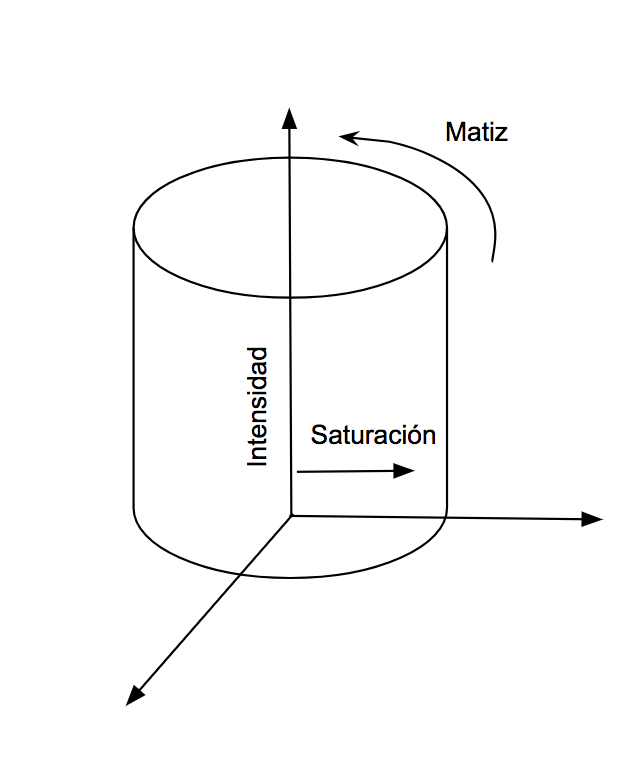
\includegraphics[width=70mm]{./figuras/diagrama-hsi.png}
\caption{Representación espacial del modelo de color HSI}
\label{img:hsi-diagrama}
\end{figure}

La representación cilíndrica de HSI se muestra en la Figura \ref{img:hsi-diagrama}, donde el ángulo en el sistema de coordenadas polar se corresponde con el matiz, la saturación se corresponde con la distancia radial y la intensidad esta dada por la distancia a lo largo del eje perpendicular al plano de coordenadas polares~\cite{OrtizZamora2002}.
\addsymbol{symbol:H}\addsymbol{symbol:S}\addsymbol{symbol:I}
Los valores de matiz ($H$), saturación ($S$) e intensidad ($I$) son calculados a partir de los valores RGB.

La transformación básica a partir de RGB de la matiz $H$ con rango [0,1] esta dada por:
\begin{equation}
H = \cos^{-1}\left[\frac{\frac{1}{2}\left[\left(r-g\right)+\left(r-b\right)\right]}{\sqrt{\left(r-g\right)^{2}+\left(r-b\right)\left(g-b\right)}}\right],
\end{equation}
donde si $b > g$, entonces $H=1-H$.

Posteriormente se calculan los valores de $S$ e $I$ como sigue:
\begin{equation}
S = 1-3\frac{min\left(r,g,b\right)}{r+g+b},
\end{equation}
\begin{equation}
I = \frac{r+g+b}{3}.
\end{equation}
\subsubsection{CIELab}
La \gls{cie} presentó el espacio de color $L^*a^*b^*$. Este espacio de color fue diseñado para que los colores que sean visualmente similares se representen en el espacio a unas distancias proporcionales a las diferencias visuales entre ellos, si la medida de distancia correcta es empleada~\cite{hanbury2001mathematical}. CIELab a diferencia del espacio RGB es independiente al dispositivo en el cual se representa.

\begin{itemize}
\addsymbol{symbol:l*}\addsymbol{symbol:a*}\addsymbol{symbol:b*}
\item $L^*$ representa la luminiscencia.
\item $a^*$ codifica la sensación rojo-verde, con $a^*$ positivo indicando un color rojo y $a^*$ negativo indicando un color verde.
\item $b^*$ codifica la sensación amarillo-azul, con $b^*$ positivo indicando un color amarillo y $b^*$ negativo indicando un color azul.
\end{itemize}
La representación espacial de CIELab se muestra en la Figura \ref{img:cielab-diagrama}. La escala de grises se encuentra en el eje $a^*=0$ y $b^*=0$ con negro en $L^*=0$ y blanco en $L^*=100$.

\begin{figure}[h!]
\centering
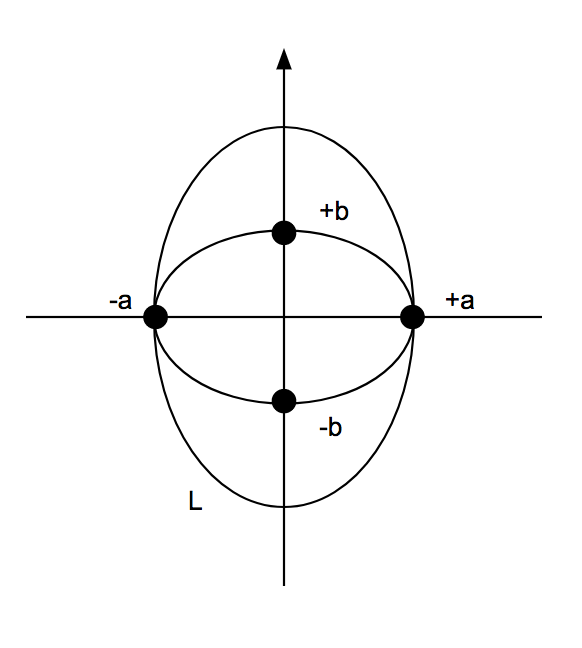
\includegraphics[width=80mm]{./figuras/diagrama-cielab.png}
\caption{Representación espacial del espacio de color CIELab}
\label{img:cielab-diagrama}
\end{figure}

La transformación del espacio de color RGB a \gls{cielab}~\cite{connolly1997study}, esta dada por la ecuación:
\addsymbol{symbol:x} \addsymbol{symbol:y} \addsymbol{symbol:z}
\addsymbol{symbol:r} \addsymbol{symbol:g} \addsymbol{symbol:b}
\begin{equation}
\begin{aligned}
X = 0,4303r + 0,3416g + 0,1784b, \\
Y = 0,2219r + 0,7068g + 0,0713b, \\
Z = 0,0202r + 0,1296g + 0,9393b. \\
\end{aligned}
\end{equation}
Se aplica la ecuación de CIELab
\begin{equation}
\label{formula:cielab}
\begin{aligned}
L^{*} = 116f\left(\frac{Y}{Y_{0}}\right) -16, \\
a^{*} = 500\left[f\left(\frac{X}{X_{0}}\right) - f\left(\frac{Y}{Y_{0}}\right)\right],\\
b^{*} = 200\left[f\left(\frac{Y}{Y_{0}}\right) - f\left(\frac{Z}{Z_{0}}\right)\right],
\end{aligned}
\end{equation}
donde
\addsymbol{symbol:f}\addsymbol{symbol:q}
\begin{equation}
\begin{aligned}
f(q) = \sqrt[3]{q} ~~ \text{si } q> 0,008856,\\
f(q) = 7,787q + \frac{16}{116}  ~~\text{si } q\leq 0,008856,
\end{aligned}
\end{equation}
para
\begin{equation}
\begin{aligned}
X_{0}=95.047, Y_{0}=100.00, Z_{0}=108.883,
\end{aligned}
\end{equation}
que son los valores del iluminante, en este caso el iluminante D65~\cite{connolly1997study}, 
el cual es un iluminante estándar de uso común definido por la CIE.
\addsymbol{symbol:elab}

La diferencia de color entre dos coordenadas en el espacio CIELab, $(L^{*}_{1},a^{*}_{1},b^{*}_{1})$ y $(L^{*}_{2},a^{*}_{2},b^{*}_{2})$ se define como $\Delta E_{Lab}$ y esta dada por la distancia Euclidiana~\cite{robertson1977cie}.
\begin{equation}
\label{formula:eucli}
\Delta E_{Lab} = \sqrt{(\Delta L^{*})^2 + (\Delta a^{*})^2 +(\Delta b^{*})^2},
\end{equation}
donde 
\addsymbol{symbol:deltal}
\addsymbol{symbol:deltaa}
\addsymbol{symbol:deltab}
\begin{equation}
\Delta L^{*} = L^{*}_{1} - L^{*}_{2},
\Delta a^{*} = a^{*}_{1} - a^{*}_{2},
\Delta b^{*} = b^{*}_{1} - b^{*}_{2}.
\end{equation}

\section{Resumen}

En este capítulo se presentaron los espacios de color más prevalentes en la literatura que serán utilizados para implementar la transformada de watershed y comparar el rendimiento de los mismos.
